%
% File: outline.tex
% Author: Oliver J. H. Feighan
% Description: Thesis outline
% Thesis outline
%
%\let\textcircled=\pgftextcircled
\chapter{Introduction}
\label{chap:intro}

\initial{P}hotosynthesis is the bedrock of life on this planet. It is often the 
first step in the food chain, establishing ecosystems from a near unlimited source 
of sunlight. Photosynthetic organisms formed around 3.5 billion years ago \cite{Blankenship2010}.
Some of the most studied photosynthetic organisms include purple bacteria \cite{Cogdell2021, Mirkovic2016, Cleary2013, Curutchet2016, Sundstro1999, Damjanovic2002, Konig2012}, 
which use light harvesting complexes (LHCs) to absorb and stabilize energy from 
light and transfer this energy to reaction centres (RCs) \cite{Klamt2008}. Chemical
potential energy from the RCs is eventually used to produce adenosine triphosphate (ATP),
the transportable energy source required for many biochemical processes. These complexes
are extremely efficient, with the light harvesting complex 1 and 2 (LH1, LH2) found 
in purple bacteria being around 95\% efficient at transferring the electronic energy 
to charge separation \cite{Tretiak2000}.

Many types of LHCs exist, differing by the type of chlorophyll pigments as well 
as structural features. Most often these complexes are formed of repeated units.
For example the LH2 complex found in \emph{Rhodoblastus acidophilus} is formed of 
a trimer unit with two bacterial chlorophyll \emph{a} (BChla) chromophores in close 
proximity, with parallel porphyrin planes, and a third chromophore perpendicular 
at a greater separation (shown in figure \ref{fig:LH2_subunit}) \cite{Cogdell2006}. 
This unit is then repeated to form a circular structure with anywhere between an
8-10 fold symmetry depending on the species of bacterium (see figure \ref{fig:LH2_rings})
\cite{Mallus2018, Cleary2013}. The efficiency of LHCs is dependent on many factors 
including this structure, the conformations of the chromophores, and their effect 
on nuanced electronic energy transfer mechanisms \cite{Harel2012}.

\begin{figure}
	\centering 
	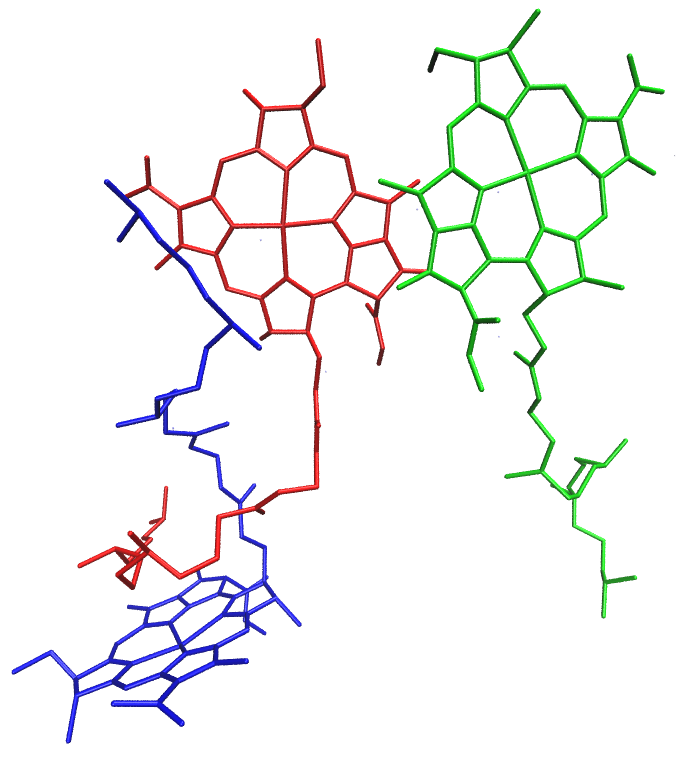
\includegraphics[scale=0.3]{chapters/1_introduction/subunit.png}
	\caption{The trimer chlorophyll unit found in LH2, coloured by ring type (red and green
	for B850a and B850b, blue for B800).}
	\label{fig:LH2_subunit}
\end{figure}

\begin{figure}
	\centering 
	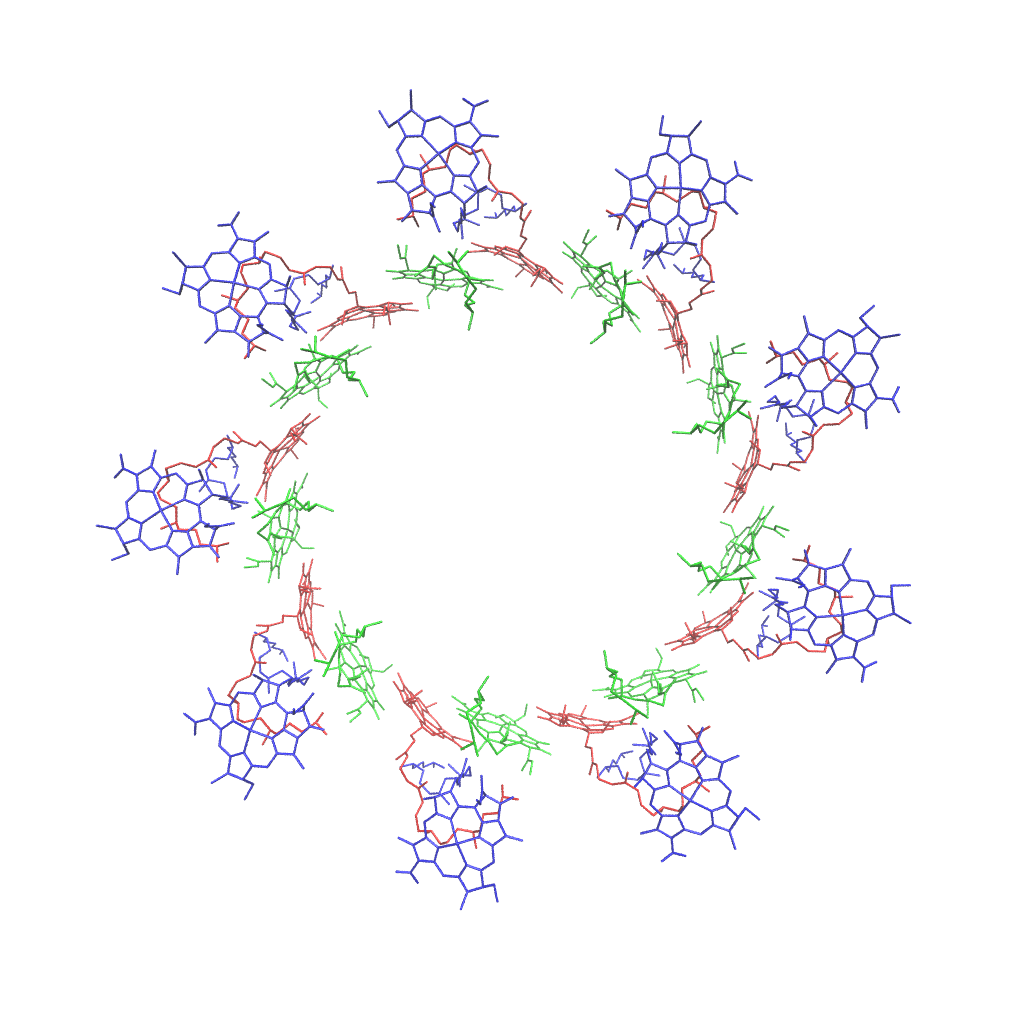
\includegraphics[scale=0.3]{chapters/1_introduction/ring_assign.png}
	\caption{The complete chlorophyll system found in LH2, coloured by ring type
	(red and green for B850a and B850b, blue for B800). This particular structure 
	has a 9-fold symmetry, giving the circular ring structures.}
	\label{fig:LH2_rings}
\end{figure}

Detailed computational study of these structures has been possible since the first
reports on high level resolution of crystal structures \cite{Mcdermott1995, Koepke1996} 
and has produced a wealth of analysis. Many of these studies explore the complex 
mechanisms of electronic energy transfer as well as environmental effects of the 
protein scaffold on spectroscopic properties of LHCs, including insights into LH2
exciton states\cite{Calhoun2009}, energy transfer timescales\cite{Akhtar2020, Moulisova2009},
excitation diffusion lengths\cite{Amarnath2016}, energetic fine-tuning by local 
effects such as H-bonding\cite{Mennucci2019, Montemayor2018} and more \cite{SlaMa2020, Jang2015, Curutchet2016, Mirkovic2016}. 
These studies show that the effects of the protein which occur on the atomistic
level are an important aspect to capture in LHC models.

Theoretical studies on LHCs can compliment experimental studies by altering factors
that are not possible to control in lab-based studies. For example, two-dimensional
electronic-vibrational (2DEV) spectra on the LH2 protein (in this case from spinach), 
produced experimentally \cite{CLewis2016}, can probe the electronic excitation energy
transfer between chlorophylls. Whilst many features in the protein scaffold can 
be proposed as origins for experimentally observed phenomena, such as amino acid
side chain carbonyl groups for characteristic 1670 $\text{cm}^{-1}$ vibrational 
modes \cite{Barth2000}, complete assignment of all effects is not possible from 
experiment alone. Atomistic theoretical studies can pinpoint these properties, probing
effects such as conformational distortions, hydrogen bonding, coordination state
and polarization in site environments \cite{CLewis2016, Lewis2015}.  

Theoretical discussion of electronic energy transfer requires models for the excited
states of LHCs. The ideal model would be a full electronic Hamiltonian of the entire
LHC complex and it's environment. However due to the size of these systems it is
usually necessary to reduce the number of degrees of freedom \cite{Mallus2018, SlaMa2020}. 
For example in LH2 the chlorophyll molecules alone contain 3780 atoms with an additional 
~6000 atoms for the entire scaffold \cite{Neugebauer2008, Cherezov2006}. Including
a membrane and explicit solvent can quickly lead to system sizes in the region of
300,000 atoms \cite{Mennucci2019}. Treating every electron in this system is not
a sensible (or as yet possible) approach.

Evidently a naive approach of using electronic structure methods that describe molecular
excited states (e.g. DFT) is not tenable for LHC models. Instead exciton models 
are used. Excitons are defined as a bound state of an electron and electron hole,
where energy can be transferred without the movement of charge \cite{Craig1968, Scholes2006}.
Characterizing excitons by the interaction between the electron and its hole gives
two limits (i.e. a strong or weak interaction). A weak interaction (often in materials
with a high dielectric constant) leads to Wannier-Mott excitons \cite{Wannier1937},
common in semiconductors and bulk metallic materials. Conversely a strong interaction
(low dielectric constant) give Frenkel excitons \cite{Frenkel1931}, common in organic
systems (i.e. LHCs), which are more localized due to the strong force between electron 
and hole. As LHCs have low dielectric constants the Frenkel model is more appropriate.
Often Frenkel exciton are modelled in a Davydov formalism, giving a Frenkel-Davydov 
exciton framework\cite{Davydov1964}. This framework constructs an exciton Hamiltonian 
from intra-site energies and inter-site interactions, reducing the degrees of freedom
of the Hamiltonian from the entire complex to just single chromophores. A more formal
description is given in the next chapter.

The Frenkel exciton Hamiltonian can either be constructed from time-independent
parameters, fitted to experimental data or calculated theoretical values, or as 
functions of LHC geometry and/or time. A good example of using static parameters 
to model LH2 is Tretiak's work on calculating LH2 ring energy transfer rates \emph{et al.} \cite{Tretiak2000}.
In this work a collective electronic oscillator model was used to calculate chromophore 
energies and couplings, and subsequently build a Frenkel exciton framework which
accurately reproduced B800-B850 and B800-B800 energy transfer rates. This model 
shows how a minimalist response theory and statical approach can produce physically
meaningful results. However, to recover a truly atomistic treatment of LHCs it is
necessary to take the functional (and dynamic) approach and treat every chromophore
geometry variation, which can be far more expensive to calculate as Hamiltonians 
are required for every frame in a time series of LHC geometries. This approach also
comes with the caveat that methods used to construct the exciton Hamiltonian have 
to be quite accurate as geometry variations are usually very small, although these
small variations are also used to justify a time-averaged parameters. The resultant
range of accuracy from geometry variations is $\sim$0.2--0.4 eV \cite{Renger2013, Hansen2019}.

Often atomistic LHC models fall into a regular pattern, recently reviewed by Mennucci 
\emph{et al.}\cite{Cignoni2022}. Electronic structure calculations are used to
produce excited state properties for individual sites, which in turn are used to
construct Frenkel exciton Hamiltonians, ultimately giving the excited states of
the whole LHC. The main design choices for LHC models are in choosing methods for
these steps. The first choice is which electronic structure and excited state method 
to use to calculate intra-site properties, and then the second choice is how to 
use these properties to construct the exciton Hamiltonian. The decisions on these
choices are highly dependent on the level of detail required for the exciton system
(atomistic or coarse grain), and the number of unique Hamiltonians required (how 
many frames of molecular dynamics (MD) are used). For a coarse-grain model, where
the full geometry of the chlorophyll system is not important, then more approximate 
methods can be used.

For a truly atomistic approach often density functional theory (DFT) and linear 
response methods (time-dependent DFT or TD-DFT) are used to calculate single site
properties \cite{Cignoni2022}. Due to the size of chlorophyll molecules, using high
level methods such as SCS-CC2 and EOM-CCSD would not be reasonable. Even with TD-DFT
methods only a limited number of explicit Hamiltonians could be constructed before
outstripping a reasonably accessible cost. If a large number of LHC geometries need 
to be calculated then further approximations are necessary.

This trade-off between computational expense and fine-grain accuracy is the main
issue in designing physical models for the excited state of LHCs. Often it is found
that while coarse-grain models are good enough for large scale phenomena, smaller
details are lost when using low-level electronic structure and response calculations.
Previous studies have suggested some solutions to this problem and these are discussed
below, along with their limitations. These limitations sketch out the potential 
for a new kind of excited state LHC model, which is the main investigation of this
work.

\section{Efficient Excited State Methods}
\label{sec:efficient_response_methods}

The most obvious solution to this scaling problem is to make the electronic structure 
and excited state calculations more efficient, often done at the expense of accuracy.
Many recent studies use tight binding methods such as TD-DFTB or ZINDO to calculate
transition properties \cite{Jurinovich2015, Olbrich2010, Curutchet2011, Curutchet2012}. 
These methods can include environmental effects (such as continuous solvent models 
or point charge embedding) and are implemented in a wide range of electronic structure
packages (for example Gaussian \cite{Gaussian16}, DFTB+ \cite{Hourahine2020}, entos/qcore \cite{Manby2019},
ORCA \cite{Neese2012, Neese2018}, and TeraChem \cite{Seritan2020, Seritan2021}). 
Comparisons of low-level (TD-DFTB), mid-level (i.e. TD-DFT) and high-level (multireference
configuration-DFT and complete active-space SCF) methods have demonstrated that 
often lower level methods are accurate enough to investigate mechanisms in LHCS
(for example the role of carotenoids \cite{Andreussi2015}, the interaction of excited
states in the $Q$ band \cite{Hansen2019} and the role of functional groups on excitation
energies in chlorophylls \emph{f}, \emph{d} and \emph{a} \cite{Poddubnyy2021}) but
it is necessary for benchmarking of these methods as not all give reliable results \cite{Dahlbom2005}.
Particularly for studies on chlorophyll, TD-DFB and ZINDO are popular choices when
requiring a large number of calculations \cite{Cignoni2022}.

Designing tight-binding models can be challenging due to the balance between accuracy
and the number of parameters that need to be fit. This issue has been explored thoroughly 
by the xTB methods developed by Grimme \emph{et al.} \cite{Bannwarth2020}. A more
in-depth discussion of all of these methods is given in the next chapter, however
as their excited state method (referred to as sTDA-xTB) is relevant to the discussion
on LHC models, an outline and discussion of this method are given below.

\subsection{sTDA-xTB}
\label{subsec:stda_xtb}
sTDA-xTB ("simplified Tann-Dancoff Approximation - eXtended Tight Binding") is a
method in the family of xTB methods developed by the Grimme and coworkers and is
parameterised for transition properties \cite{Grimme2016}. The accuracy in calculating
transition energies with this method is very good with the error compared to high-level 
methods such as SCS-CC2 being between 0.34 - 0.48 eV dependent on the benchmark.

Similar to other xTB methods, sTDA-xTB is based on tight-binding electronic structure
that uses empirically fitted parameters and a minimal basis set. Discussed in more
detail in chapter \ref{chap:background_theory}, tight-binding schemes assume small
variations in electron density that remove the need to treat core electrons explicitly
and often only consider valence electron effects. It was trained on a set of highly
accurate coupled cluster and density functional theory excitation energies, as well
as atomic partial charges for inter-electronic interactions.

Unlike other xTB methods, basis set function coefficients in sTDA-xTB are dependent
on coordination number of the atom centres. This makes basis functions far more 
flexible, which could only be achieved with fixed basis functions by using diffuse
or additional orbitals in the basis set. It also uses two sets of parameterized 
basis sets - a smaller valence basis set (VBS) and an extended basis set (XBS).
Whilst this approach reduces the cost of having larger basis sets, it makes calculating
the gradients of transition properties much more difficult.

The two basis sets are used to construct formally similar Fock matrix elements,
although in practice they use different global parameters. The core Hamiltonian
is similar to other DFTB methods that use a self-consistent charge (SCC) method 
to obtain molecular orbital (MO) coefficients. It is given by

\begin{equation}
\bra{\psi_\mu} H^{\text{EHT, sTDA-xTB}} \ket{\psi_\mu}= \frac{1}{2} \left(k^l_\mu k^{l'}_\nu\right) \frac{1}{2} \left(h^l_\mu h^{l'}_\nu\right) S_{\mu\nu} - k_T \bra{\psi_\mu}\hat{T}\ket{\psi_\nu}
\end{equation}
%
where $\mu,\nu,l,l'$ are orbital and shell indices, $k^l_\mu$ are shell-wise 
H{\"u}ckel parameters, $h$ are effective atomic-orbital energy levels, $S_{\mu\nu}$
is the overlap of orbitals $\mu$ and $\nu$, $k_T$ is a global constant and $\hat{T}$
is the kinetic energy operator. The charges used in the inter-electronic repulsion 
function are given by charge model 5 (CM5) \cite{Marenich2012} charges for the XBS
Fock matrix. These are calculated using Mulliken charges obtained from diagonalizing
the Fock matrix with the VBS. The charges for the initial VBS Fock matrix are based
on Gasteiger charges \cite{Gasteiger1978}, modified by the parameterized
electronegativities of atoms in the system.

The whole process for determining molecular orbitals can be summarized as:
\begin{enumerate}
	\item Calculate modified Gasteiger charges for the first initial guess
	\item Diagonalize Fock matrix in the VBS to get the first set of Mulliken charges
	\item Compute CM5 charges
	\item Diagonalize Fock matrix in the VBS again for final set of Mulliken charges.
	\item Recalculate CM5 charges with this final set, and diagonalize the Fock matrix in the XBS. 
	\item The molecular orbital coefficients from this are then fed to the response theory.
\end{enumerate}

The response theory for this method is based on previous work in the Grimme group
on the simplified Tamm-Dancoff Approximation \cite{Grimme2013}. There are several
approximations made between full linear response theory and the sTDA method. First
is the Tamm-Danncoff approximation, where some transition characters are ignored
(a more formal description is given in section \ref{subsubsec:Tamm_Dancoff}). The
second approximation is to use a Mataga-Nishimoto-Ohno-Klopman (MNOK) method to 
calculate two electron integrals instead of explicitly calculating them \cite{Nishimoto1957, Ohno1964, Klopman1964}.

Transition charges are used to calculate these MNOK integrals. These charges $q^A_{nm}$
(centred on atom $A$ and associated with the transition $ n \rightarrow m$) are
computed using a Löwdin population analysis

\begin{equation}
q_{nm}^A = \sum_{\mu \in A} C^\prime_{\mu n} C^\prime_{\mu m},
\end{equation}

where the transformed coefficients $C^\prime_{\mu n}$ are given by orthogonalizing
the original MO coefficients $\textbf{C}$

\begin{equation}
\textbf{C}^\prime = \textbf{S}^{\frac{1}{2}} \textbf{C},
\end{equation}

and $\mu$ is an index that runs over the atomic orbitals (AO). The MO coefficients
are the solution of diagonalizing the Fock matrix (from the Roothaan-Hall equations,
see equation \ref{eq:roothaan_hall}).

The approximations to full two electron integrals are given by damped charge-charge
interactions - this approach will be discussed in more detail in chapter \ref{chap:chl_xtb}
as it is a crucial part of designing a new excited state method for chlorophyll systems. 

Lastly the single particle excited space used to construct the full transitions
is truncated more than that of normal TD-DFT. This reduces the number of elements
that need to be calculated, reducing the time taken for diagonalization whilst also
capturing a broad enough range of excitation energies. 

The sTDA-xTB method is reported as having excellent accuracy against benchmarked
data, and has been used to generate absorption spectra and other properties for 
large systems \cite{Grimme2016, Seibert2019, Wilbraham2018, Verma2022, HeathApostolopoulos2019}. 
Whilst some early benchmarking of sTDA-xTB shows its ability to match experimental
absorption spectra \cite{Grimme2016}, and can be extended to predict experimental
absorption spectra very well small metallo-organic complexes and \cite{Seibert2019},
recent work has used sTDA-xTB to screen a wide range of compounds in high-throughput
methods \cite{Wilbraham2018}, as well as the basis for a $\Delta$-ML model (where
the error between a high (TD-DFT) and low level (sTDA-xTB) method is calibrated) \cite{Verma2022}.
In this way much of the work reporting sTDA-xTB accuracy has been performed on a 
range of systems, and does not concern smaller geometry variations of a single system. 
The latter is more important for LHCs, as it is the variations in chlorophyll geometries
that cause variations in the exciton system and these are relatively small \cite{Sirohiwal2020}.
As sTDA-xTB prediction of chlorophyll systems has not been reported much before, 
especially with regard to conformer variations, it is difficult to say whether it
would be better than previously used tight-binding methods. It may be better to start
from methods that do have accurate correlations with system geometries, such as
TD-DFT, and work from these to retain accuracy. This strategy is explored in the
next section on statistical method based on high-level data to generate exciton
Hamiltonian matrix elements.

\section{Statistical Methods}
\label{sec:stats_methods}

Making approximations in constructing the exciton framework is an alternative option
to response method approximations. One of the simplest ways of doing this is by 
using static parameters fit from experimental or calculated data \cite{Cory1998, Hu1997, Tretiak2000}. 
These are referred to as static in this work as the parameters do not vary between 
frames in a time series of LHC geometries. Using these static Hamiltonians negates
any variation in intra-chromophore or protein scaffold geometry, but can still produce
good predictions of physical phenomena, such as an estimate of the population of
excited states \cite{Cory1998, Hu1997} and B800-B850 energy transfers. As said, 
this approach breaks down when more atomistic considerations are necessary.

Over a long timescale where the full conformation space is well sampled, exciton
Hamiltonians can be constructed from distributions of chromophore transition properties
(i.e. excitation energies and transition densities) \cite{Stross2016}. These properties
are approximately distributed along a normal distribution when taken from a set 
of uncorrelated structures. The mean and standard deviations can then be used to 
define a distribution function that can be limitlessly sampled to construct Hamiltonians
without the need for explicit calculations on separate structures. The Hamiltonians
could utilize functions that take into account inter-chromophore geometries, for
example by calculating coupling values from a distribution function of transition
dipole magnitudes, or use distributions for all elements of the Hamiltonian matrix.

However, these methods are ill-suited for dynamic studies where structures at different
times are correlated, which is an important consideration for LH2 \cite{Papiz2003}.
Recently machine-learning methods have been reported that give time-dependent Hamiltonians
but still without the need for expensive calculations.

\subsection{Machine-Learning For Exciton Models}
\label{subsec:machine_learning} 

Machine-learning models have been used in many areas of computational chemistry,
especially in areas where both large amounts of data and well-defined metrics make 
it easy to train  methods \cite{Dral2020, Behler2011, Westermayr2020, Schutt2019, Sajjan2022}.
For example, models that predict forcefield constants and atomization energies can
be readily made as root mean square deviations of atomic positions and mean absolute 
errors in energies are well-defined metrics  \cite{Rupp2012, Dick2019, Scherer2020}.
Similar to sTDA-xTB, ML models can be used for screening in high-throughput workflows 
- a particularly relevant example of this is on screening organic photovoltaics 
considering these systems have $\pi$-conjugation chemistry similar to chlorophyll \cite{Zhao2022}.
At their heart, these methods are similar to the static statistical methods that
have already been used for LH2 exciton systems, as they rely on parameters fitted to
high level data. However the incorporation of atomic geometry information and machine-learning
techniques can give time dependent models, as discussed below.

In 2016 H\"{a}se \emph{et al.} reported on a multi-perceptron or neural network (NN)
model that predicts the \Qy transition for chlorophyll molecules \cite{AspuruGuzik2016}.
Using this model, as well as fitted parameters for the exciton coupling, it was 
possible to calculate exciton population dynamics, as well as spectral densities
for chlorophyll sites in the FMO light harvesting complex. Similar to other models
a "Coulomb matrix" \cite{Rupp2012a, Montavon2013} is used as descriptor of the chlorophyll
systems defined as 

\begin{equation}
	M_{AB} = 
	  \begin{cases}
		\frac{1}{2} Z^{2.4} \text{ for } A = B\\
		\frac{Z_A Z_B}{\left\lvert \mathbf{R}_A - \mathbf{R}_B\right\rvert} \text{ for } A \neq B
	  \end{cases}
\end{equation}
%
where $Z_A$ is some measure of the atomic charge on atom $A$, and $R_A$ is the position
vector. It can be seen that the off-diagonal elements are simply the Coulombic interactions,
and diagonal elements are a polynomial of the atomic charges. This descriptor is
popular due to the similarity in information that an electronic structure calculation
would start from, namely the positions and nuclear charges of atoms \cite{Raghunathan2022}.

The Coulomb matrix is then used as an input for a neural network model. A neural 
network is a series of matrix operations applied to input data that overall acts
as a non-linear function. In this way NN models are conceptually similar to biological 
neurons, which take in electrical signals and through some mechanism can be activated
to send out a different signal. The outputs of each operation is described as a 
layer, with each element in a layer referred to as a node (i.e. nodes stack vertically
into layers, layers stack horizontally into the network). The first and last layers 
are named input and output layers and any steps in-between referred to as "hidden" 
layers \cite{Rumelhart1986}.

\begin{figure}
	\centering
	\begin{neuralnetwork}[height=4]
        \inputlayer[count=3, bias=true, title=Input\\layer]
        \hiddenlayer[count=4, bias=false, title=Hidden\\layer 1] \linklayers
        \hiddenlayer[count=3, bias=false, title=Hidden\\layer 2] \linklayers
        \outputlayer[count=2, title=Output\\layer] \linklayers
	\end{neuralnetwork}
	\caption{A schematic of a neural network showing how inputs, such as the
	(flattened) Coulomb matrix, are ordered into nodes (green and yellow) and can
	be used to generate outputs (red nodes). The blue nodes between these layers
	constitute the "hidden layers". Each arrow leading to a node represents a matrix
	multiplication and activation function application. The values in the output
	layer for models discussed in the text would be \Qy transition energies or atom
	centered transition charges.}
	\label{fig:neural_network}
\end{figure}

A layer can be any distinct vector of values. For example, flattening the Coulomb 
matrix into a 1D vector gives the input layer, and the \Qy transition energy and 
dipole moment the output vector (of 2 elements). The vector $\mathbf{V}_{(n+1)}$
at layer index $n+1$ is given by multiplicating the previous layer, $\mathbf{V}_{(n)}$,
with a coefficient matrix $c$ and applying some function $f$

\begin{equation}
	\mathbf{V}_{n+1} = f(\mathbf{c}_n \mathbf{V}_n)
\end{equation}
%
where the coefficient matrices $\mathbf{c}_n$ are fitted to give the smallest error
between the output layer values and some target data (i.e.\Qy energies), and the
function $f$ can amplify beneficial values in nodes, mimicking the activation of
biological neurons (giving the name activation functions). The activation functions  
are also parameterised, with the most common functions being sinusoidal ($f(\mathbf{V}_n)=cos(m \mathbf{V}_n)$), 
sigmoid ($f(\mathbf{V}_n)=\frac{m_1}{m_2 + e^{m_3 \mathbf{V}_n}}$), linear 
($f{\mathbf{V}}_{n}=m \mathbf{V}_{n}$) or rectified linear unit ($f(\mathbf{V}_{n})=\text{max}\left(0, m \mathbf{V}_{n} \right)$). 
The coefficient matrices $\mathbf{c}_n$, and parameters used in the activation functions
$m$ or $m_k$, are fit by a back-propagation method, again parameterized - these fitting
parameters are referred to as hyper-parameters and have to be optimized to give 
the best coefficient matrix using supervised learning techniques such as a systematic
grid-search. Other considerations such as over-fitting also need to be taken into account.
The brief explanation of NNs here glosses over more practical considerations, and
creating these models takes in-depth knowledge and experience to achieve good results.

The H\"{a}se NN model predicted \Qy transition energies with around a 0.3 meV error
for all of the 8 sites in the FMO complex \cite{AspuruGuzik2016}. This is exceptionally
accurate, supporting the idea that models lacking in chemical nuance, but still 
given atomic positions and nuclear charges, have all the information necessary to
predict transition energies. It is noted in this work that the root mean squared 
deviations (RSMD) of Nitrogen atom positions compared to the energy-minimized crystal 
structure correlate well with excited state properties. This implies that structural
information is key to get transition properties correct and should be a primary 
consideration when discussing models for chlorophyll transition properties. Exciton
properties, such as the time series of exciton populations, were also well reproduced
using these \Qy energies, although the coupling parameters were taken from other
fits and not from a NN method.

Another method, developed by Farahvash \emph{et al.}, utilized both neural networks
and kernel ridge regression (KRR) to predict both site energies as well as exciton 
coupling parameters, giving a completely time dependent exciton Hamiltonian \cite{Farahvash2020}. 
KRR is another machine-learning method that can be understood as two processes \cite{Hastie2009}. 
First is the ridge regression, which is similar to a linear regression model but 
with an additional factor to account for co-linear relationships between inputs.
Regression models are multivariate linear models that follow the form

\begin{equation}
	f^\prime\left(\mathbf{X}\right) = \mathbf{X} \mathbf{\beta}
\end{equation}
%
where $f^\prime\left(\mathbf{X}\right)$ are the predicted values of some metrics $f\left(\mathbf{X}\right)$ 
(i.e. \Qy energy or exciton coupling value), $\mathbf{X}$ is the matrix of information
used to predict the value $f$ (i.e. flattened Coulomb matrix, referred to as the feature
matrix) and $\beta$ is a set of fitted coefficients that minimize the value $\left\lvert f^\prime \left( \mathbf{x}\right) - f \left(\mathbf{x}\right)\right\rvert$.
The matrix $\mathbf{\beta}$ can be found by minimizing the square of this value, 
known as the least-squares method. However this can lead to expensive terms when
calculating the inner product of the feature matrix. Here the "kernel trick" is 
used to make these terms easier to calculate. This rearranges the minimization of
regression coefficients so that the inner products are not required, but requires 
a new function that compares the similarity of features. Ultimately, the function 
$f^\prime$ becomes

\begin{equation}
	f_{\text{KRR}}^\prime = \sum^{N_x}_j \beta_j k\left(\mathbf{x}, x_j\right)
\end{equation}
%
where the $N_x$ is the size of the feature vector $\mathbf{x}$ (which in the linear
model is stacked to form the matrix $\mathbf{X}$), and $k$ is the kernel function.
Often this is a gaussian function of the feature vector

\begin{equation}
	k\left(\mathbf{x}, x_j\right) = \text{exp}\left(\frac{-\left(\mathbf{x}-x_j\right)^2}{2\sigma^2}\right)
\end{equation}
%
where $\sigma$ is a fitted parameter \cite{Rasmussen2006}. Again these parameters 
are optimised by a systematic search through values, similar to the grid search
referenced earlier.

In the Farahvash work a KRR model was developed for both the excitation energies
and exciton coupling parameters. However it was found that a NN model predicted 
exciton couplings with greater accuracy, which was attributed to the more complex 
conformational space. This NN model calculated atomic centered transition charges,
which were then used to calculate coupling elements with small error against higher 
level methods. This corroborates another study on exciton coupling methods that
argues that transition charge based methods are accurate enough for almost all needs \cite{Kenny2016}.

These machine-learning models show that it is possible to generate time and geometry
dependent functions that give either transition properties needed to construct exciton
Hamiltonians or the full Hamiltonians themselves. However there are some issues 
with this approach. In contrast to the sTDA-xTB method, machine learning models 
do not use any formalism that treats the electronic structure explicitly. This makes 
it difficult to include any other effects such as continuous solvent models or point
charge embedding that are often used in LHC quantum mechanics / molecular mechanics
(QM/MM) models. Some models do use QM/MM methods to generate training data but this
would only lead to pigeonholing the optimized model to the QM/MM setup used. Additionally
machine-learnt models would not able to calculate any other properties than those 
they are taught - for example the models that return \Qy transition energies would 
not be able to return ground state energies, a trivial task for fully quantum methods
like TD-DFT. In short, a machine learning method will only be as good as the method
it is trained on and cannot predict anything not built into its architecture. There
are also some practical considerations as well when designing these models, such
as the requirement of in-depth knowledge of machine-learning methods to retrain 
models. The cost of generating enough data to train these models is also very high.
For example the number of data points required to train the H\"{a}se and Farahvash 
models was on the order of $10^4$ and $10^5$ respectively. The compute walltime 
for such datasets would be in the hundreds or thousands of hours. In summary, whilst these
models are accurate enough to reliably make time-dependent Hamiltonians they are
 limited by both their designs and their construction cost.

\section{GPU Acceleration}
\label{sec:gpu_acceleration}

An alternative approach to these problem would be to accelerate high-level calculations.
This is possible with various established techniques such as multi-node parallelism
(an early example is the parallelization of GAMESS \cite{Fletcher2000}) but as this 
requires the exclusive use of many (dozens) of CPUs this is not a favourable option 
to take. Instead a better approach is to use graphical processing units (GPUs), 
which have been used to accelerate many different types of molecular chemistry simulations \cite{Pandey2022}.
Programs written for GPUs can partition a limited number of basic operations over 
a massive number of parallel components, and this is exploited to parallelize the
bottleneck of expensive calculations \cite{McIntosh-Smith2013}. For example to accelerate
TD-DFT calculations of chlorophyll excited states, the bottleneck would be evaluating
the electron integrals necessary to construct the Casida equation (see section \ref{subsec:tddft})
Further afield, examples of GPU usages include the evaluating forces in MD simulations
from classical equations as well as the matrix operations for NNs discussed above \cite{Ufimtsev2008, Friedrichs2009, Wu2012}.

This approach does not require any parameter optimization or new formalism but does
require appropriate hardware (GPU cards) and programs that can partition on GPUs
correctly. However, this is a common feature on high performance computers. GPU-acceleration
has been used in many studies and is a popular way of drastically increasing system 
sizes while keeping computing time down \cite{Seritan2021}. One of the first and 
still popular electronic structure programs specifically designed for GPUs is TeraChem
\cite{Seritan2020}, with earlier programs focussing on molecular mechanics programs 
such as OpenMM \cite{Eastman2017} and Amber \cite{Salomon-Ferrer2013}.

Previous work has used GPU-based programs to study LH2, using full TD-DFT calculations
to construct Frenkel exciton Hamiltonians for every frame of an LH2 MD simulation \cite{Sisto2014a, Sisto2017}.
The workflow was similar to exciton frameworks discussed above, using transition
properties on sites to evaluate Hamiltonian elements - all of the transition properties
were calculated using TD-DFT with the $\omega\text{PBEh}$ functional and 6-31G basis
set. These calculations were accelerated using GPU hardware with Terachem so the
compute wall-time would be similar to tight-binding and machine-learning methods. 
With this acceleration it was also possible to calculate transition properties on
larger aggregates of chlorophyll molecules, such as a combination of the two subunits
shown in figure \ref{fig:LH2_subunit}. There was an average error of 8 meV when
benchmarking the exciton framework against TD-DFT calculations on these hexamer
complexes \cite{Sisto2014a}. Absorption spectra predicted by full TD-DFT and the
exciton model were also very similar. The benefit of using a more efficient method
to calculate TD-DFT data is showcased by the production of a non-adiabatic dynamic
simulation with gradient terms of the exciton system being calculated on-the-fly
or 300 fs. This required the construction of the Frenkel exciton Hamiltonian to
be on the timescale of other gradient methods (i.e. force-fields or some semi-empirical 
tight-binding methods).

Whilst computing the electron integral terms with GPUs requires far less computing 
time, storing these values is a major issue \cite{Sisto2014a}. This is due to the
lightweight memory capacity on GPU cards, and even makes recalculation of some integrals
more efficient than storage. This means that a larger basis sets or more complicated
density functionals may be too expensive to use. Therefore trying to calculate high-level
data may be an issue for a more detailed study. It may be argued that accelerating 
the generation of high-level data would be better done by machine-learning methods.
Similar to the other methods discussed, it is clear there are benefits and compromises
with GPU acceleration.

\section{Aims}
\label{sec:possible_novel_methods}

The underlying issue of LHC models is clear - the systems are too large to explicitly
calculate all transition properties required when using high level methods. Making
well-chosen approximations has found success in solving some parts of this issue
but ubiquitously at some other expense. The sTDA-xTB method (and other tight-binding
methods) are efficient but generally not accurate enough to give reliable results 
like TD-DFT or higher-level methods. Machine-learning methods are accurate and efficient
but not extendable, use large amounts of expensive high level training data, and
require a good understanding of machine-learning methods. Accelerating calculations 
with GPUs could also be used but may still come up against memory issues which limits 
the extent of the basis set and density functional.

These shortcomings sketch out the need for a method that is efficient, accurate,
extendable, memory light and easy to reproduce. The work presented in this thesis
explores whether novel excited state methods in conjunction with efficient electronic 
structure methods could constitute a good method for LHCs models - this strategy 
is similar to the sTDA-xTB approach although with a more specialized scope. Most 
of this work is based on tight-binding approaches as these fulfill most of the criteria 
set out above except accuracy, making them the optimal starting place. In order 
to assay the usability of these novel approaches it is necessary to benchmark transition 
properties against established methods (explored in chapters \ref{chap:dscf} and 
\ref{chap:chl_xtb}) as well as provide case studies of calculating full LHC models 
(chapters \ref{chap:excitons} and \ref{chap:LH2}). A description of all of the common 
theories used (DFT, DFTB/xTB, TD-DFT and Frenkel-Davydov models) is given in the 
next chapter.

\section{Outline}
\label{sec:outline}

The remainder of this thesis is structured into 6 more chapters. This chapter has
introduced and discussed how efficient LHC models have been explored in previous 
work and the issues that have been discovered. The following chapter summarizes 
existing methods that are used throughout this work.

\textbf{Chapter \ref{chap:dscf}} is an investigation of whether mean-field methods,
such as \dscf and eigenvalue difference, can reliably predict transition properties 
and particularly addresses their suitability for treating for bulk chlorophyll transition
properties. It also discusses how the underlying level of electronic structure theory
affects the accuracy of transition properties.

\textbf{Chapter \ref{chap:chl_xtb}} uses these findings to inform the design of 
Chl-xTB, a novel approach to calculating biochromophore excited states. While it
is not a general purpose method, its application to the \Qy transition of chlorophyll 
shows excellent performance. It fulfills the criteria set out above, obtaining transition
properties with great efficiency whilst also achieving an accuracy comparable to 
TD-DFT methods.

\textbf{Chapter \ref{chap:excitons}} demonstrates the application of chl-xTB to chlorophyll 
dimer systems, using an exciton framework that can extend to multiple chlorophyll
systems such as light harvesting proteins. Comparison to high level theories show 
that the new workflow can be expected to give good properties beyond monomer systems. 
With this workflow it starts to be possible to make novel arguments about light 
harvesting system phenomena. Specifically, the new workflow is used to explain how
charge separation (which can potentially lead to unwanted fluorescence quenching) 
in chlorophyll dimers is suppressed by the LH2 protein scaffold.

\textbf{Chapter \ref{chap:LH2}}, then reports on applying the novel method to the
whole LH2 chlorophyll system. The high level of detail and efficiency is used to 
access low-frequency spectral densities of the entire LH2 complex, offering new
insight into the effect of complex-wide vibrations on exciton transport dynamics.

The last chapter, \textbf{Chapter \ref{chap:discussion}}, discusses the conclusions
from the previous results chapters. Investigations such as applying the novel excited 
state method to systems beyond chlorophyll are discussed, as well as alterations 
to the exciton benchmarking and framework. More applications to LH2 and other light 
harvesting systems are proposed.

